\documentclass[11pt,a4paper]{article}

\usepackage[
    a4paper,
    left=15mm,
    right=15mm,
    top=30mm,
    bottom=25mm,
    headheight=25mm
]{geometry}
\usepackage{graphicx}
\usepackage{polski}
\usepackage[utf8]{inputenc}
\usepackage{enumerate}
\usepackage{comment}
\usepackage{fancyhdr}
\usepackage{hyperref}
\usepackage{indentfirst}
\usepackage{multirow}
\usepackage{multicol}
\usepackage{float}
\usepackage{amsmath}
\usepackage{fancyhdr}
\usepackage{wrapfig}
\usepackage{layout}
\usepackage{textcomp}
\usepackage[center]{caption}
\usepackage{subcaption}
\usepackage{siunitx}

\sisetup{output-exponent-marker=\ensuremath{\mathrm{e}}}

\renewcommand{\baselinestretch}{1.18}
\renewcommand\thesubfigure{\roman{subfigure}}

\pagestyle{fancy}
\fancyhead[L]{
    
\includegraphics[scale=0.16]{../agh_logo_text_asym.jpg}
}
\fancyhead[R]{
    Lab 1 - Predykaty geometryczne | Łukasz Dragon 14.10.2024
}

\begin{document}
\section{Wstęp}
Celem ćwiczenia była implementacja, testy i wizualizacja
podstawowego predykatu geometrycznego - określenia po 
której stronie prostej znajduje się punkt.
\subsection{Wstęp teoretyczny}
Niech punkty $a = (a_x,a_y)$ i $b = (b_x, b_y)$ wyznaczają jednoznacznie
prostą $k$. 

Pozycja punktu $c = (c_x, c_y)$ względem $k$ zależy od wyznacznika
$det(a, b, c)$, który możemy wyliczyć na dwa sposoby:
\begin{equation}
\begin{split}
    det(a, b, c) =&
    \begin{vmatrix}
        a_x & a_y & 1 \\
        b_x & b_y & 1 \\
        c_x & c_y & 1
    \end{vmatrix}
    \\
    \text{lub}
    \\
    det(a, b, c) =&
    \begin{vmatrix}
        a_x - c_x & a_y - c_y \\
        b_x - c_x & b_y - c_y
    \end{vmatrix}
\end{split}
\end{equation}

Zależność jest następująca:
\begin{equation}
\begin{split}
    det(a, b, c) > 0 &\iff c \text{ leży po lewej } k
    \\
    det(a, b, c) < 0 &\iff c \text{ leży po prawej } k
    \\
    det(a, b, c) = 0 &\iff c \text{ leży na } k
\end{split}
\end{equation}

\begin{figure}[H]
    \centering
    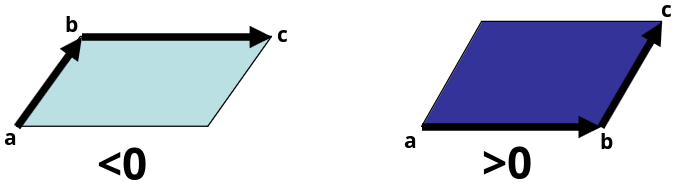
\includegraphics[scale=0.75]{res/example.png}
    \caption{Wizualizacja zależności jako pola równoległoboku}
\end{figure}

\subsection{Specyfikacja narzędzi i sprzętu}
Wszystkie potrzebne obliczenia zostały wykonane
przy użyciu interpretera języka Python wersji 3.12.
Ponadto, w celu wygenerowania zbiorów punktów 
i sprawdzenia bibliotecznych funkcji wyliczania
wyznacznika, użyłem biblioteki \verb|numpy|.
Wykresy i wizualizacja wyników została przygotowana
za pomocą narzędzia przygotowanego przez koło naukowe
Bit. Kod znajduje się w załączonym pliku.

Przedstawione wyniki zostały wygenerowane na komputerze
z systemem operacyjnym Debian 12 i procesorem Intel Core i5-8250U 1.6 GHz.

\pagebreak

\section{Realizacja obliczeń}

Obliczenia rozpocząłem od przygotowania czterech zbiorów losowych punktów:

\begin{figure}[H]
    \centering
    \begin{subfigure}[b]{0.46\textwidth}
        \centering
        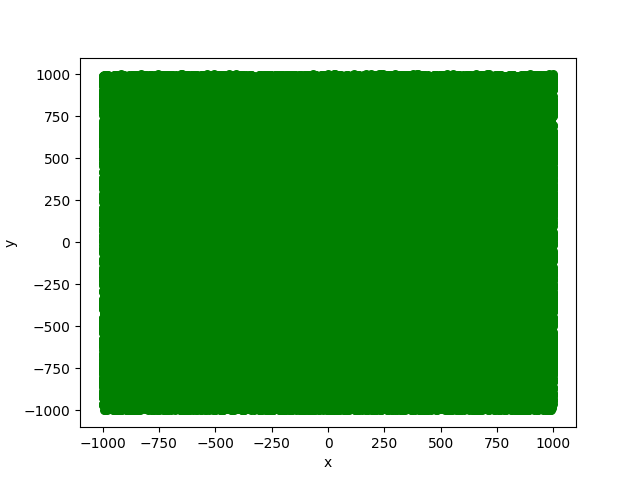
\includegraphics[scale=0.5]{res/rec1.png}
        \caption{
            Zbiór A 
            \\ 
            \footnotesize$10^5$ punktów o współrzędnych
            \\
            z przedziału $[-1000, 1000]$.
        }
    \end{subfigure}
    \begin{subfigure}[b]{0.46\textwidth}
        \centering
        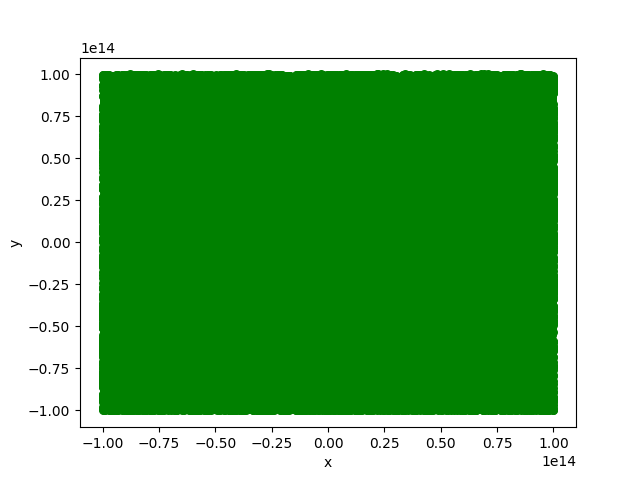
\includegraphics[scale=0.5]{res/rec2.png}
        \caption{
            Zbiór B 
            \\ 
            \footnotesize$10^5$ punktów o współrzędnych
            \\
            z przedziału $[-10^{14}, 10^{14}]$.
        }
    \end{subfigure}
    \begin{subfigure}[b]{0.46\textwidth}
        \centering
        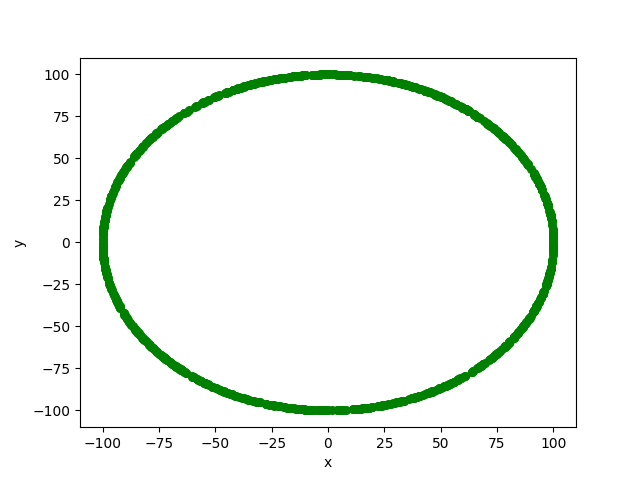
\includegraphics[scale=0.5]{res/cir.png}
        \caption{
            Zbiór C
            \\
            \footnotesize$1000$ punktów na okręgu: $x^2 + y^2 = 100$.
            \\
            ~
            \\
            ~
        }
    \end{subfigure}
    \begin{subfigure}[b]{0.46\textwidth}
        \centering
        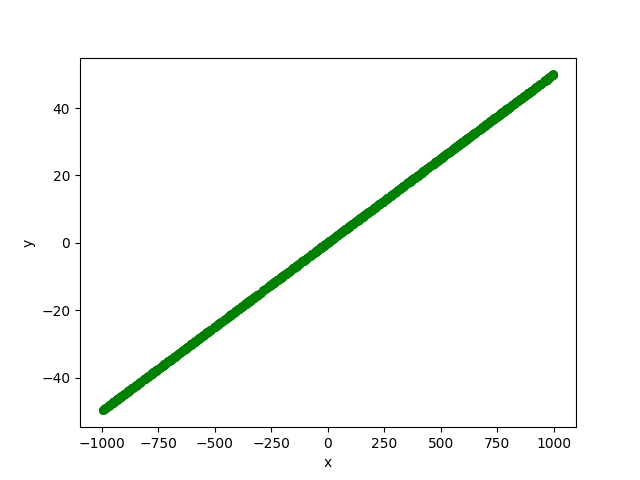
\includegraphics[scale=0.5]{res/lin.png}
        \caption{
            Zbiór D
            \\
            \footnotesize$1000$ punktów o współrzędnej $x\in[-1000, 1000]$,
            \\
            leżących na prostej wyznaczonej przez punkty 
            \\
            $a = (-1, 0)$, $b = (1, 0.1)$. 
        }
    \end{subfigure}
    \caption{Wygenerowane zbiory}
\end{figure}

Następnie każdy z tych zbiorów podzieliłem względem prostej wyznaczonej
przez punkty $a = (-1, 0)$, $b = (1, 0.1)$ korzystając z różnych 
implementacji liczenia wyznacznika, tolerancji dla zera i precyzji
liczb zmiennoprzecinkowych. Funkcje, używane przeze mnie do liczenia 
wyznacznika, to:
\begin{multicols}{2}
\begin{itemize}
    \item \begin{verbatim*}mat_det_2x2\end{verbatim*}
    (implementacja w załączonym pliku)
    \item \begin{verbatim*}mat_det_2x2_lib\end{verbatim*}
    (funkcja biblioteczna \verb|numpy.linalg.det|)
    \item \begin{verbatim*}mat_det_3x3\end{verbatim*}
    (implementacja w załączonym pliku)
    \item \begin{verbatim*}mat_det_3x3_lib\end{verbatim*}
    (funkcja biblioteczna \verb|numpy.linalg.det|)
\end{itemize}
\end{multicols}
\section{Wyniki}
Tabele 1, 2, 3, 4 i Rysunki 3, 4, 5, 6 przedstawiają wyniki podziałów punktów
dla każdego zbioru w zależności od funkcji, tolerancji 
($\varepsilon = 0, 10^{-14}, 10^{-12}, 10^{-10}, 10^{-8}$) 
i precyzji zmiennych (\verb|float64| lub \verb|float32|).
Za wyniki w tabelach przyjmuję ilość punktów zakwalifikowanych
kolejno po lewej, po prawej i na prostej.

Na wykresach punkty leżące na lewo i prawo
od prostej będą zaznaczane kolejno na zielono i pomarańczowo,
a punkty leżące na prostej - na fioletowo. Sama prosta jest zaznaczona
na czerwono.

\subsection{Zbiór A}
\begin{table}[H]
    \centering
    \begin{tabular}{|l|l|l|l|l|l|l|}
    \hline
        \textbf{Funkcja} & \textbf{Po lewej} & \textbf{Po prawej} & \textbf{Na prostej} & \textbf{Po lewej} & \textbf{Po prawej} & \textbf{Na prostej} \\ \hline
        $\varepsilon=\num{0},\num{1e-14},...$ & \multicolumn{3}{>{\ttfamily\arraybackslash}c|}{float64} & \multicolumn{3}{>{\ttfamily\arraybackslash}c|}{float32} \\ \hline
        \verb|mat_det_3x3| & 50084 & 49916 & 0 & 50084 & 49916 & 0 \\ \hline
        \verb|mat_det_3x3_lib| & 50084 & 49916 & 0 & 50084 & 49916 & 0 \\ \hline
        \verb|mat_det_2x2| & 50084 & 49916 & 0 & 50084 & 49916 & 0 \\ \hline
        \verb|mat_det_2x2_lib| & 50084 & 49916 & 0 & 50084 & 49916 & 0 \\ \hline
    \end{tabular}
    \caption{Rozkład punktów dla zbioru A}
\end{table}

Dla każdej sprawdzonej tolerancji, precyzji i funkcji wyniki podziału
są identyczne i nie występują żadne błędy wynikające z reprezentacji
liczb rzeczywistych za pomocą liczb zmiennoprzecinkowych.

Na Rysunku 3 znajduje się wykres podziału punktów, który jest
taki sam dla wszystkich sprawdzonych przypadków:

\begin{figure}[H]
    \centering
    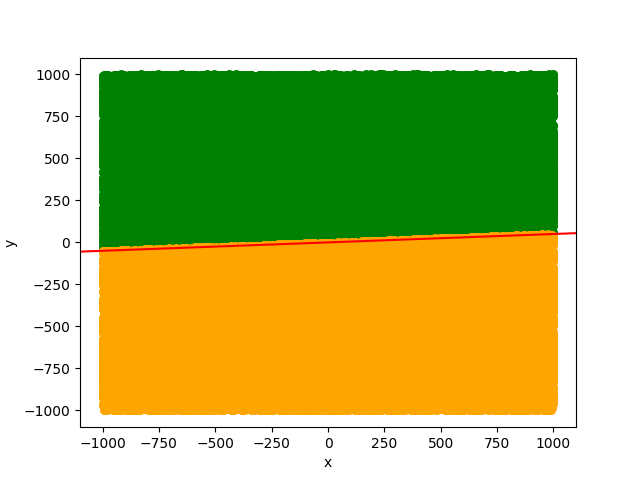
\includegraphics[scale=0.5]{res/rec1_mat_det_2x2_float32_1e-14.png}
    \caption{Wykres rozkładu punktów w zbiorze A}
\end{figure}

\subsection{Zbiór B}
\begin{table}[H]
    \centering
    \begin{tabular}{|l|l|l|l|l|l|l|}
    \hline
        \textbf{Funkcja} & \textbf{Po lewej} & \textbf{Po prawej} & \textbf{Na prostej} & \textbf{Po lewej} & \textbf{Po prawej} & \textbf{Na prostej} \\ \hline
        $\varepsilon = \num{0}$ & \multicolumn{3}{>{\ttfamily\arraybackslash}c|}{float64} & \multicolumn{3}{>{\ttfamily\arraybackslash}c|}{float32} \\ \hline
        \verb|mat_det_3x3| & 50120 & 49880 & 0 & 50120 & 49880 & 0 \\ \hline
        \verb|mat_det_3x3_lib| & 50120 & 49880 & 0 & 50120 & 49880 & 0 \\ \hline
        \verb|mat_det_2x2| & 50116 & 49876 & 8 & 0 & 0 & 100000 \\ \hline
        \verb|mat_det_2x2_lib| & 50116 & 49875 & 9 & 6545 & 6621 & 86834 \\ \hline
        $\varepsilon = \num{1e-14}$ & \multicolumn{3}{>{\ttfamily\arraybackslash}c|}{float64} & \multicolumn{3}{>{\ttfamily\arraybackslash}c|}{float32} \\ \hline
        \verb|mat_det_3x3| & 50120 & 49880 & 0 & 50120 & 49880 & 0 \\ \hline
        \verb|mat_det_3x3_lib| & 50120 & 49880 & 0 & 50120 & 49880 & 0 \\ \hline
        \verb|mat_det_2x2| & 50116 & 49876 & 8 & 0 & 0 & 100000 \\ \hline
        \verb|mat_det_2x2_lib| & 50116 & 49875 & 9 & 6545 & 6621 & 86834 \\ \hline
        $\varepsilon = \num{1e-12}$ & \multicolumn{3}{>{\ttfamily\arraybackslash}c|}{float64} & \multicolumn{3}{>{\ttfamily\arraybackslash}c|}{float32} \\ \hline
        \verb|mat_det_3x3| & 50120 & 49880 & 0 & 50120 & 49880 & 0 \\ \hline
        \verb|mat_det_3x3_lib| & 50120 & 49880 & 0 & 50120 & 49880 & 0 \\ \hline
        \verb|mat_det_2x2| & 50116 & 49876 & 8 & 0 & 0 & 100000 \\ \hline
        \verb|mat_det_2x2_lib| & 50116 & 49875 & 9 & 6545 & 6621 & 86834 \\ \hline
        $\varepsilon = \num{1e-10}$ & \multicolumn{3}{>{\ttfamily\arraybackslash}c|}{float64} & \multicolumn{3}{>{\ttfamily\arraybackslash}c|}{float32} \\ \hline
        \verb|mat_det_3x3| & 50120 & 49880 & 0 & 50120 & 49880 & 0 \\ \hline
        \verb|mat_det_3x3_lib| & 50120 & 49880 & 0 & 50120 & 49880 & 0 \\ \hline
        \verb|mat_det_2x2| & 50116 & 49876 & 8 & 0 & 0 & 100000 \\ \hline
        \verb|mat_det_2x2_lib| & 50116 & 49875 & 9 & 6545 & 6621 & 86834 \\ \hline
        $\varepsilon = \num{1e-8}$ & \multicolumn{3}{>{\ttfamily\arraybackslash}c|}{float64} & \multicolumn{3}{>{\ttfamily\arraybackslash}c|}{float32} \\ \hline
        \verb|mat_det_3x3| & 50120 & 49880 & 0 & 50120 & 49880 & 0 \\ \hline
        \verb|mat_det_3x3_lib| & 50120 & 49880 & 0 & 50120 & 49880 & 0 \\ \hline
        \verb|mat_det_2x2| & 50116 & 49876 & 8 & 0 & 0 & 100000 \\ \hline
        \verb|mat_det_2x2_lib| & 50116 & 49875 & 9 & 6545 & 6621 & 86834 \\ \hline
    \end{tabular}
    \caption{Rozkład punktów dla zbioru B}
\end{table}

Jak widać w Tabeli 2, wyniki są niezależne od przyjętej tolerancji.  
Jest tak, ponieważ prawdopodobieństwo znalezienia losowego punktu w zbiorze B
na naszej prostej jest astronomicznie małe. Możemy z tego wywnioskować,
że zakwalifikowanie jakichkolwiek punktów jako leżących na prostej, wynika
z błędu i niewystarczającej precyzji reprezentacji liczb w komputerze.

Pominę wyniki dla funkcji liczących wyznacznik macierzy $3\times3$,
ponieważ dzielą one nasz zbiór, tak jakbyśmy się tego spodziewali.
Najciekawsze wyniki widzimy dla wyznacznika $2\times2$, w którym pojawiają
się pierwsze błędy. Dla precyzji \verb|float64| występuje ich nieznaczna
ilość, lecz dla \verb|float32| wyniki są kompletnie błędne.

\pagebreak

Weźmy dla przykładu punkt $c = (\num{-4.5074654e+13}, \num{-4.6074136e+13})$.
Podążając algorytmem na obliczanie wyznacznika macierzy $2\times2$:
\begin{equation}
\begin{split}
    &a_x - c_x = -1 - (\num{-4.5074654e+13})
    =_{\text{\ttfamily\arraybackslash float32}}
    \num{4.5074654e+13}
    \\
    &b_y - c_y = 0.1 - (\num{-4.6074136e+13})
    =_{\text{\ttfamily\arraybackslash float32}}
    \num{4.6074136e+13}
    \\
    &a_y - c_y = 0 - (\num{-4.6074136e+13})
    =_{\text{\ttfamily\arraybackslash float32}}
    \num{4.6074136e+13}
    \\
    &b_x - c_x = 1 - (\num{-4.5074654e+13})
    =_{\text{\ttfamily\arraybackslash float32}}
    \num{4.5074654e+13}
    \\
    &(a_x - c_x)(b_y - c_y) - (a_y - c_y)(b_x - c_x)
    =_{\text{\ttfamily\arraybackslash float32}}
    0
\end{split}
\end{equation}
Widzimy więc, że reprezentowalne wartości wokół $\pm10^{13}$, 
są dla precyzji \verb|float32| na tyle rzadkie, iż nie jesteśmy
w stanie rozróżnić bliskich siebie wartości.

Dla tego samego punktu funkcja biblioteczna zwraca jednak inną wartość:
\begin{equation}
\begin{split}
    \text{\ttfamily\arraybackslash mat\_det\_2x2\_lib}&(a, b, c) 
    = \num{3.5214574e11} > 0 
    \\
    &\text{ \footnotesize(punkt zakwalifikowany po lewej)}
\end{split}
\end{equation}
Wynika to prawdopodobnie z innej implementacji liczenia wyznacznika macierzy
i wewnętrznych optymalizacji. 

Na Rysunku 4 znajdują się podziały, w których występiły błędy: 

\begin{figure}[H]
    \centering
    \begin{subfigure}[b]{0.46\textwidth}
        \centering
        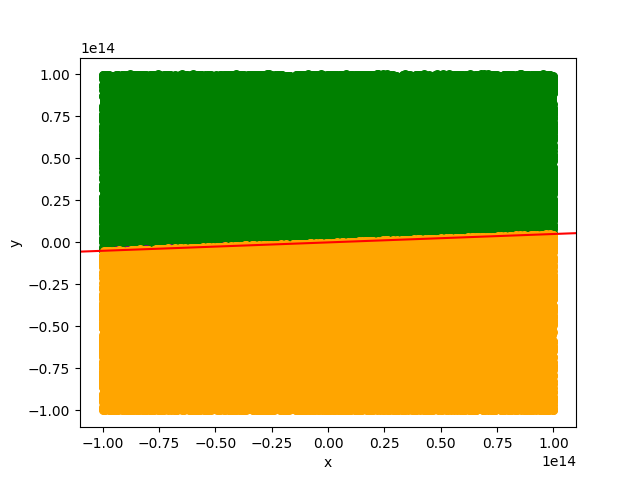
\includegraphics[scale=0.49]{res/rec2_mat_det_2x2_float64_0.png}
        \caption{\ttfamily\arraybackslash mat\_det\_2x2, float64}
    \end{subfigure}
    \begin{subfigure}[b]{0.46\textwidth}
        \centering
        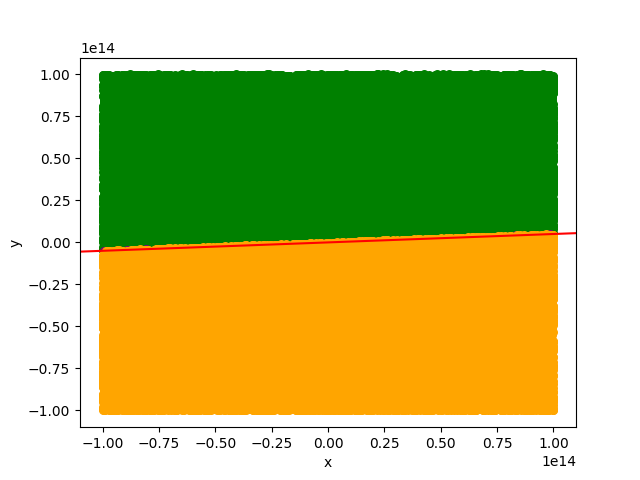
\includegraphics[scale=0.49]{res/rec2_mat_det_2x2_lib_float64_0.png}
        \caption{\ttfamily\arraybackslash mat\_det\_2x2\_lib, float64}
    \end{subfigure}
    \begin{subfigure}[b]{0.46\textwidth}
        \centering
        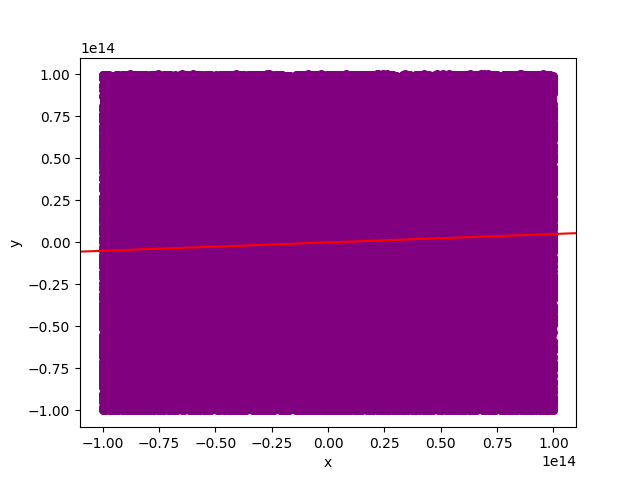
\includegraphics[scale=0.49]{res/rec2_mat_det_2x2_float32_0.png}
        \caption{\ttfamily\arraybackslash mat\_det\_2x2, float32}
    \end{subfigure}
    \begin{subfigure}[b]{0.46\textwidth}
        \centering
        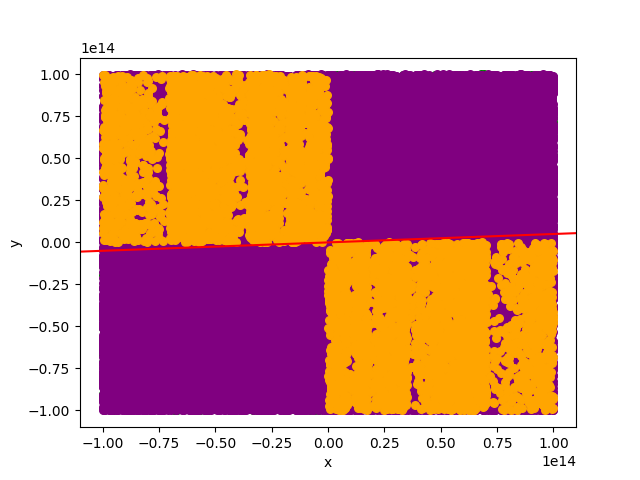
\includegraphics[scale=0.49]{res/rec2_mat_det_2x2_lib_float32_0.png}
        \caption{\ttfamily\arraybackslash mat\_det\_2x2\_lib, float32}
    \end{subfigure}
    \caption{Wykresy wybranych rozkładów punktów w zbiorze B}
\end{figure}

\subsection{Zbiór C}
\begin{table}[H]
    \centering
    \begin{tabular}{|l|l|l|l|l|l|l|}
    \hline
        \textbf{Funkcja} & \textbf{Po lewej} & \textbf{Po prawej} & \textbf{Na prostej} & \textbf{Po lewej} & \textbf{Po prawej} & \textbf{Na prostej} \\ \hline
        $\varepsilon=\num{0},\num{1e-14},...$ & \multicolumn{3}{>{\ttfamily\arraybackslash}c|}{float64} & \multicolumn{3}{>{\ttfamily\arraybackslash}c|}{float32} \\ \hline
        \verb|mat_det_3x3| & 484 & 516 & 0 & 484 & 516 & 0 \\ \hline
        \verb|mat_det_3x3_lib| & 484 & 516 & 0 & 484 & 516 & 0 \\ \hline
        \verb|mat_det_2x2| & 484 & 516 & 0 & 484 & 516 & 0 \\ \hline
        \verb|mat_det_2x2_lib| & 484 & 516 & 0 & 484 & 516 & 0 \\ \hline
    \end{tabular}
    \caption{Rozkład punktów dla zbioru C}
\end{table}

Podobnie jak dla zbioru A, wszystkie wyniki są identyczne.

Wartości współrzędnych zarówno w tym zbiorze, jak i zbiorze A, 
są małe, więc wyniki operacji zmiennoprzecinkowych na nich są
dokładniejsze. Ponadto nie sprawdzamy dokładnej wartości wyznacznika,
lecz tylko jego znak, co jeszcze bardziej ułatwia nam zdobycie
poprawnych wyników. 

Na Rysunku 5 znajduje się wykres podziału punktów, który jest
taki sam dla wszystkich sprawdzonych przypadków:

\begin{figure}[H]
    \centering
    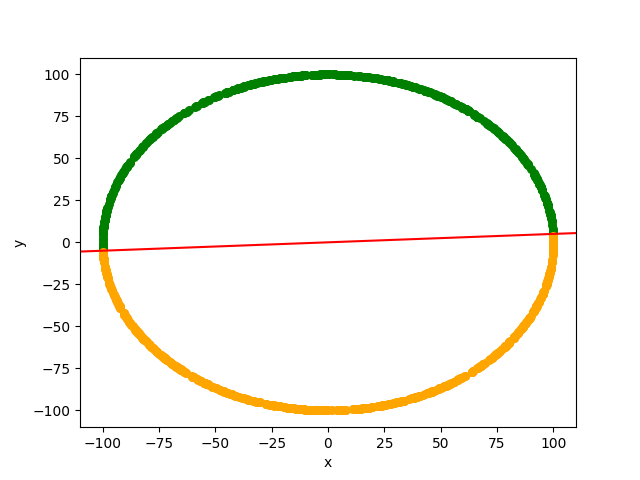
\includegraphics[scale=0.5]{res/cir_mat_det_2x2_float32_0.png}
    \caption{Wykres rozkładu punktów w zbiorze B}
\end{figure}

\subsection{Zbiór D}
\begin{table}[H]
    \centering
    \begin{tabular}{|l|l|l|l|l|l|l|}
    \hline
        \textbf{Funkcja} & \textbf{Po lewej} & \textbf{Po prawej} & \textbf{Na prostej} & \textbf{Po lewej} & \textbf{Po prawej} & \textbf{Na prostej} \\ \hline
        $\varepsilon = \num{0}$ & \multicolumn{3}{>{\ttfamily\arraybackslash}c|}{float64} & \multicolumn{3}{>{\ttfamily\arraybackslash}c|}{float32} \\ \hline
        \verb|mat_det_3x3| & 269 & 384 & 347 & 339 & 290 & 371 \\ \hline
        \verb|mat_det_3x3_lib| & 344 & 286 & 370 & 504 & 442 & 54 \\ \hline
        \verb|mat_det_2x2| & 156 & 152 & 692 & 191 & 178 & 631 \\ \hline
        \verb|mat_det_2x2_lib| & 166 & 161 & 673 & 510 & 490 & 0 \\ \hline
        $\varepsilon = \num{1e-14}$ & \multicolumn{3}{>{\ttfamily\arraybackslash}c|}{float64} & \multicolumn{3}{>{\ttfamily\arraybackslash}c|}{float32} \\ \hline
        \verb|mat_det_3x3| & 0 & 0 & 1000 & 339 & 290 & 371 \\ \hline
        \verb|mat_det_3x3_lib| & 29 & 40 & 931 & 441 & 387 & 172 \\ \hline
        \verb|mat_det_2x2| & 149 & 148 & 703 & 191 & 178 & 631 \\ \hline
        \verb|mat_det_2x2_lib| & 157 & 153 & 690 & 510 & 490 & 0 \\ \hline
        $\varepsilon = \num{1e-12}$ & \multicolumn{3}{>{\ttfamily\arraybackslash}c|}{float64} & \multicolumn{3}{>{\ttfamily\arraybackslash}c|}{float32} \\ \hline
        \verb|mat_det_3x3| & 0 & 0 & 1000 & 339 & 290 & 371 \\ \hline
        \verb|mat_det_3x3_lib| & 0 & 0 & 1000 & 431 & 374 & 195 \\ \hline
        \verb|mat_det_2x2| & 84 & 91 & 825 & 191 & 178 & 631 \\ \hline
        \verb|mat_det_2x2_lib| & 114 & 105 & 781 & 510 & 490 & 0 \\ \hline
        $\varepsilon = \num{1e-10}$ & \multicolumn{3}{>{\ttfamily\arraybackslash}c|}{float64} & \multicolumn{3}{>{\ttfamily\arraybackslash}c|}{float32} \\ \hline
        \verb|mat_det_3x3| & 0 & 0 & 1000 & 339 & 290 & 371 \\ \hline
        \verb|mat_det_3x3_lib| & 0 & 0 & 1000 & 431 & 374 & 195 \\ \hline
        \verb|mat_det_2x2| & 0 & 0 & 1000 & 191 & 178 & 631 \\ \hline
        \verb|mat_det_2x2_lib| & 0 & 0 & 1000 & 510 & 490 & 0 \\ \hline
        $\varepsilon = \num{1e-8}$ & \multicolumn{3}{>{\ttfamily\arraybackslash}c|}{float64} & \multicolumn{3}{>{\ttfamily\arraybackslash}c|}{float32} \\ \hline
        \verb|mat_det_3x3| & 0 & 0 & 1000 & 337 & 290 & 373 \\ \hline
        \verb|mat_det_3x3_lib| & 0 & 0 & 1000 & 429 & 373 & 198 \\ \hline
        \verb|mat_det_2x2| & 0 & 0 & 1000 & 191 & 178 & 631 \\ \hline
        \verb|mat_det_2x2_lib| & 0 & 0 & 1000 & 508 & 488 & 4 \\ \hline
    \end{tabular}
    \caption{Rozkład punktów dla zbioru D}
\end{table}

Zbiór D zawiera tylko wartości leżące na omawianej przez nas prostej. 
Z tego powodu, w teorii, wszystkie punkty powinny zostać zakwalifikowane
jako leżące na prostej. Jak widzimy jednak w Tabeli 4, idealne wyniki 
udało się uzyskać jedynie dla relatywnie dużych tolerancji i precyzji.
Jest tak, ponieważ ilość reprezentowalnych wartości zmiennoprzecinkowych
rośnie blisko zera. Sprawia to, że z większym prawdopodobieństwem 
wyznaczniki wyliczane są jako bardzo bliskie zeru, co wymusza na nas zwiększenie
tolerancji. 

Dla precyzji \verb|float32| natomiast wszystkie wyniki są bardzo zbliżone
do siebie, niezależnie od tolerancji. Wynika to oczywiście z jeszcze większej
niedokładności obliczeń. Uzyskanie idealnego podziału wymagałoby więc od nas
zwiększenia tolerancji.

Na Rysunku 6 znajdują się wykresy wybranych przeze mnie rozkładów, 
które moim zdaniem najlepiej obrazują różne niedokładności w wynikach.

\begin{figure}[H]
    \centering
    \begin{subfigure}[b]{0.46\textwidth}
        \centering
        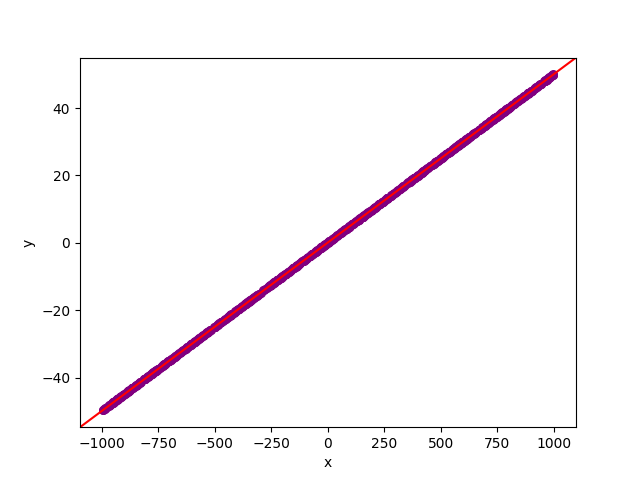
\includegraphics[scale=0.4]{res/lin_mat_det_3x3_float64_1e-10.png}
        \caption{\ttfamily\arraybackslash mat\_det\_3x3 float64 $\varepsilon=\num{1e-10}$}
    \end{subfigure}
    \begin{subfigure}[b]{0.46\textwidth}
        \centering
        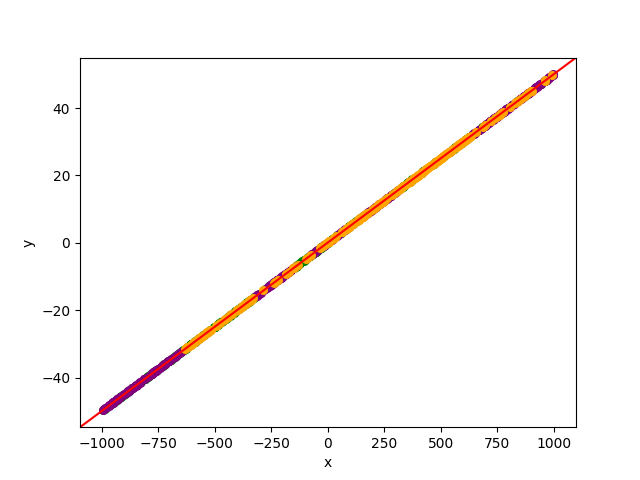
\includegraphics[scale=0.4]{res/lin_mat_det_3x3_float32_1e-10.png}
        \caption{\ttfamily\arraybackslash mat\_det\_3x3 float32 $\varepsilon=\num{1e-10}$}
    \end{subfigure}
    \begin{subfigure}[b]{0.46\textwidth}
        \centering
        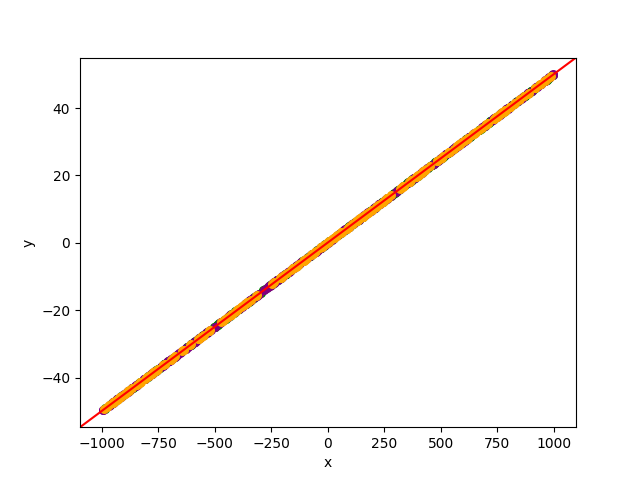
\includegraphics[scale=0.4]{res/lin_mat_det_3x3_lib_float64_0.png}
        \caption{\ttfamily\arraybackslash mat\_det\_3x3\_lib float64 $\varepsilon=\num{0}$}
    \end{subfigure}
    \begin{subfigure}[b]{0.46\textwidth}
        \centering
        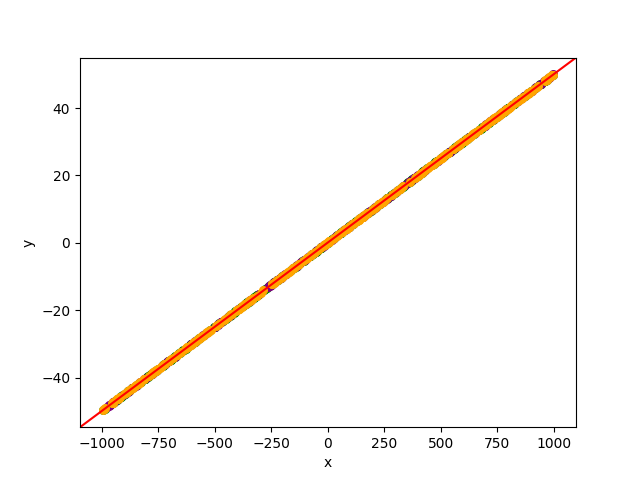
\includegraphics[scale=0.4]{res/lin_mat_det_3x3_lib_float32_1e-10.png}
        \caption{\ttfamily\arraybackslash mat\_det\_3x3\_lib float32 $\varepsilon=\num{1e-10}$}
    \end{subfigure}
    \begin{subfigure}[b]{0.46\textwidth}
        \centering
        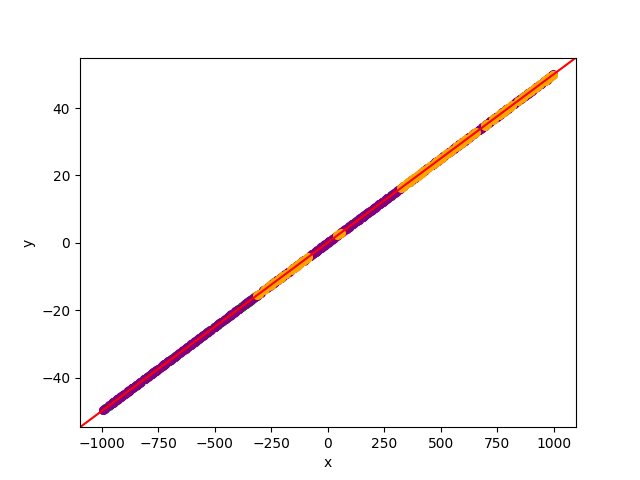
\includegraphics[scale=0.4]{res/lin_mat_det_2x2_float64_1e-14.png}
        \caption{\ttfamily\arraybackslash mat\_det\_2x2 float64 $\varepsilon=\num{1e-14}$}
    \end{subfigure}
    \begin{subfigure}[b]{0.46\textwidth}
        \centering
        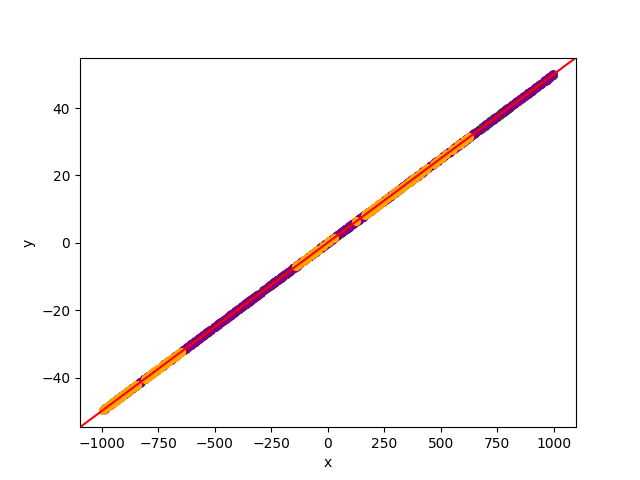
\includegraphics[scale=0.4]{res/lin_mat_det_2x2_float32_1e-10}
        \caption{\ttfamily\arraybackslash mat\_det\_2x2 float32 $\varepsilon=\num{1e-10}$}
    \end{subfigure}
    \begin{subfigure}[b]{0.46\textwidth}
        \centering
        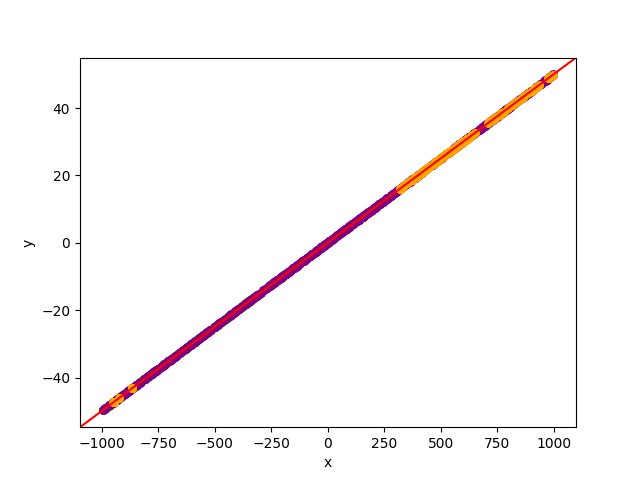
\includegraphics[scale=0.4]{res/lin_mat_det_2x2_lib_float64_1e-12.png}
        \caption{\ttfamily\arraybackslash mat\_det\_2x2\_lib float64 $\varepsilon=\num{1e-12}$}
    \end{subfigure}
    \begin{subfigure}[b]{0.46\textwidth}
        \centering
        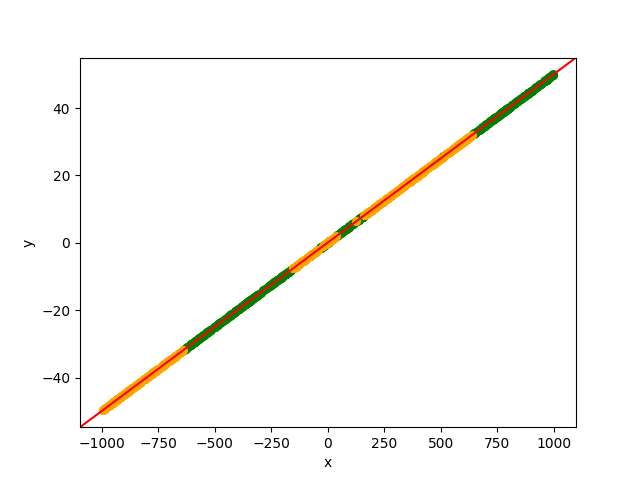
\includegraphics[scale=0.4]{res/lin_mat_det_2x2_lib_float32_1e-10}
        \caption{\ttfamily\arraybackslash mat\_det\_2x2\_lib float32 $\varepsilon=\num{1e-10}$}
    \end{subfigure}
    \caption{Wykresy wybranych rozkładów punktów w zbiorze D}
\end{figure}

\section{Podsumowanie}
Na podstawie przeprowadzonych obliczeń jesteśmy w stanie wywnioskować,
że dobranie tolerancji dla zbiorów A, B i C nie zmieniało w żaden sposób wyniku. 
W zbiorze B najważniejsza okazała się precyzja i dobór funkcji. Dla wyznaczników 
$2\times2$ nawet precyzja \verb|float64| oznaczała kilka błędów, natomiast 
dla \verb|float32| wyniki były kompletnie błedne.
Zbiór D okazał się najbardziej czuły na zmiany w tolerancji, 
która musiała być całkiem duża, żeby wyniki były w pełni poprawne.

Ostatecznie najbardziej dokładne wyniki zwracały funkcje liczące
wyznacznik macierzy $3\times3$, z czego najlepiej poradziła sobie
funkcja \verb|mat_det_3x3| będąca najprostszą implementacją
liczenia wyznacznika metodą Sarrusa. Wyjątkiem jest zbiór D przy
użyciu precyzji \verb|float32|, gdzie najbliżej poprawnych wyników była
funkcja \verb|mat_det_2x2|.

\end{document}
